\documentclass[Second Project.tex]{subfiles}

\begin{document}

\subsection{ Σύγκριση των προσεγγίσεων και ψηφία ακρίβειας }

Για την σύγκριση των παραπάνω προσεγγίσεων υπολογίζουμε το \textlatin{\textbf{RMSE}} και για τις τρεις μεθόδους για 200
σημεία στο $[-\pi, \pi]$ και καταλήγουμε στον παρακάτω πίνακα
\vspace{5mm}
\begin{center}
    \begin{tabular}{ |c|c|c| } 
     \hline
     Μέθοδος Προσέγγισης & \textlatin{RMSE} \\
     \hline
     Πολυωνυμική (\textlatin{Newton}) & $2.644882474077062e-05$ \\
     \hline
     Φυσικές Κυβικές \textlatin{Splines} & $0.0012736124616251868$ \\ 
     \hline
     Μέθοδος Ελαχίστων Τετραγώνων & $2.6267765538364208e-05$ \\
     \hline
    \end{tabular}
\end{center}
\vspace{5mm}
Απ' όπου παρατηρούμε ότι το μικρότερο \textlatin{\textbf{RMSE}} το πετυχαίνει η μέθοδος των ελαχίστων τετραγώνων 
με μοντέλο ένα πολυώνυμο 10ου βαθμού. Στην συνέχεια, την αμέσως καλύτερη επίδοση έχει η πολυωνιμκή προσέγγιση με την
μέθοδο του \textlatin{Newton} ενώ το μεγαλύτερο \textlatin{\textbf{RMSE}} το πετυχαίνουν οι φυσικές κυβικές 
\textlatin{Splines}.
\vspace{5mm}
\begin{figure}[h!]
    \centering
    \captionsetup{justification=centering}
    \subfloat{{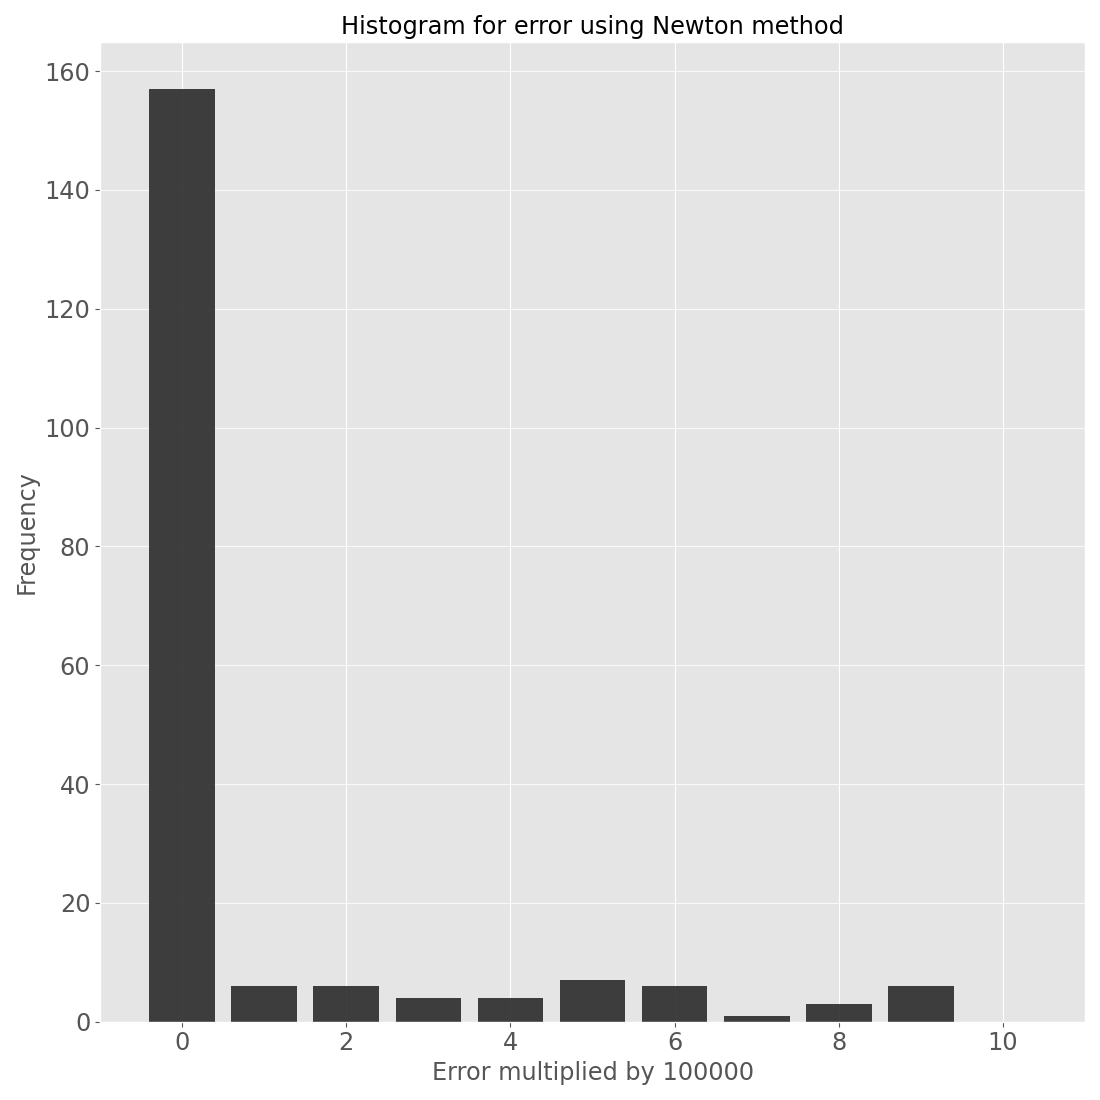
\includegraphics[scale=0.20]{newton_error_histogram.png}}}
    \quad
    \subfloat{{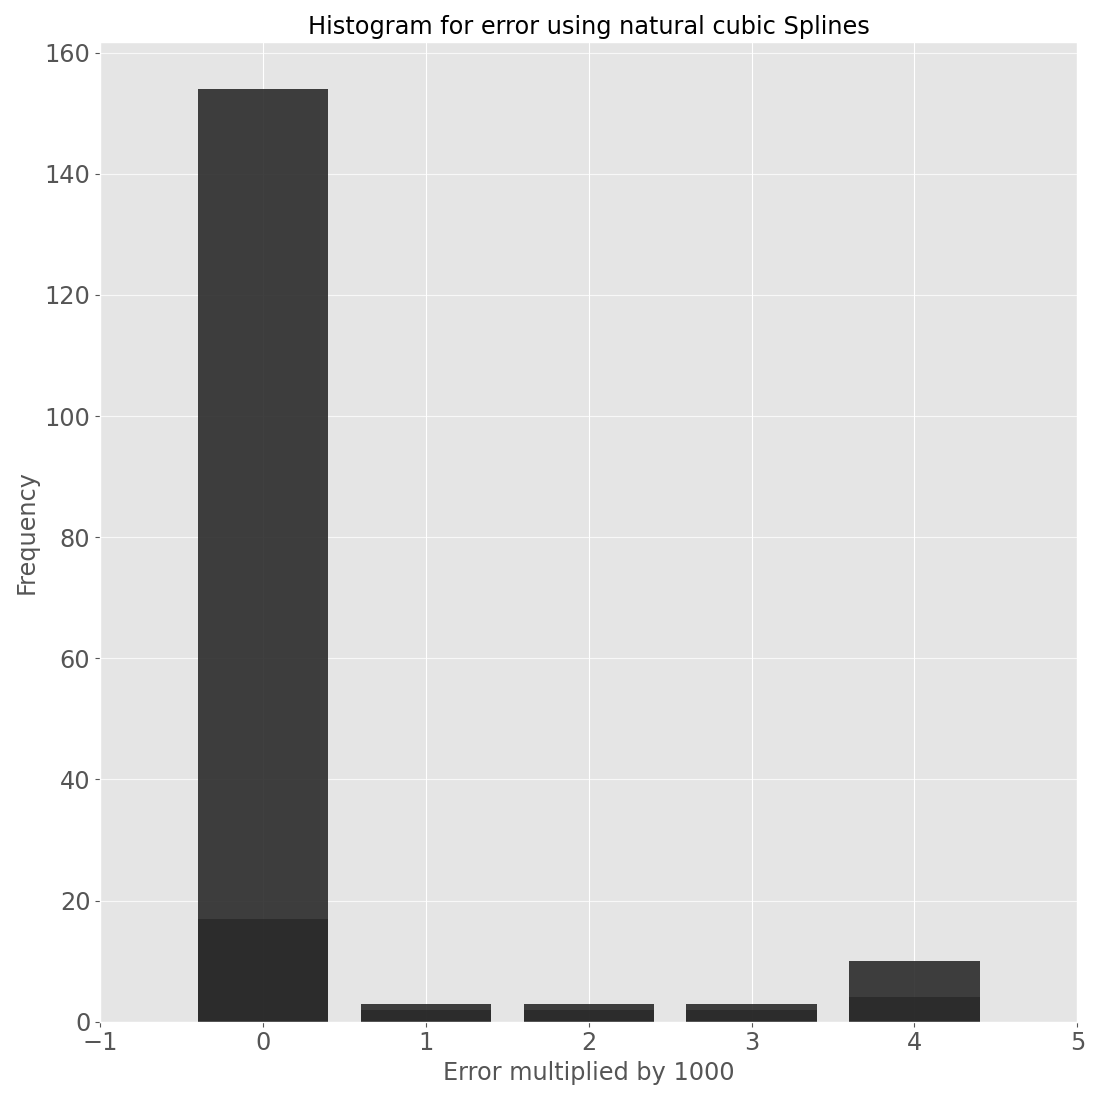
\includegraphics[scale=0.20]{splines_error_histogram.png} }}
    \caption{ Ιστογράμματα συχνοτήτων του σφάλματος προσέγγισης για 200 σημεία στο [-π, π] για τις 
    μεθόδους \textlatin{\textbf{Newton}} και \textlatin{\textbf{Splines}}.}
\end{figure}
\vspace{5px}
\begin{figure}[h!]
    \centering
    \captionsetup{justification=centering}
    \begin{center}
        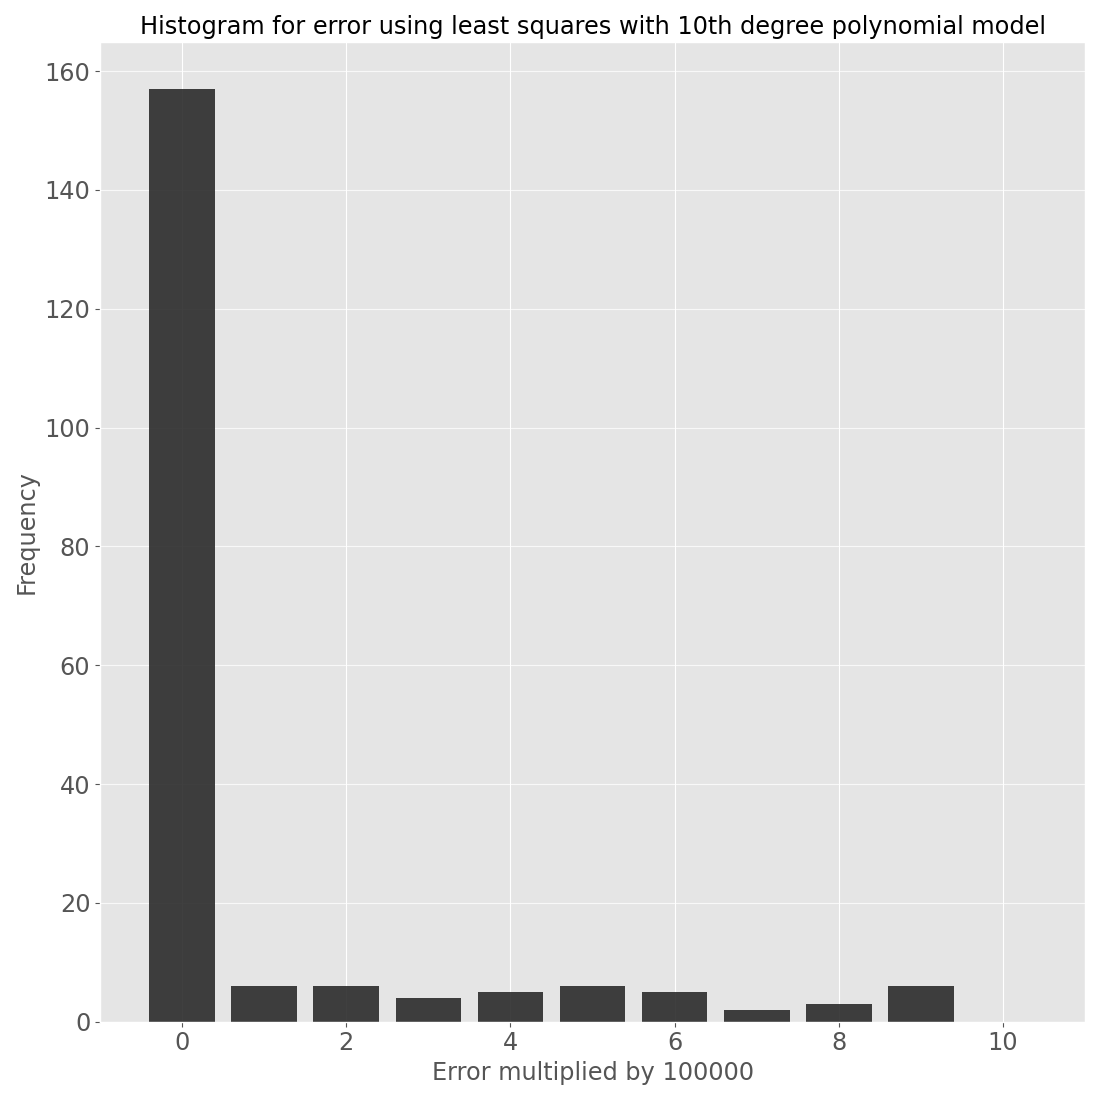
\includegraphics[scale=0.20]{least_squares_error_histogram.png}    
        \caption{ Ιστογράμματα συχνοτήτων του σφάλματος προσέγγισης για 200 σημεία στο [-π, π] για την μέθοδο των ελαχίστων τετραγώνων 
        με πολυώνυμο 10ου βαθμού.}
    \end{center}
\end{figure}
Από τα ιστογράμματα των \textit{Σχημάτων 2} και \textit{3} παρατηρούμε ότι οι μέθοδοι \textlatin{Newton} 
και ελαχίστων τετραγώνων προσεγγίζουν το ημίτονο με το σφάλμα να κυμαίνεται από $-0.00009$ εώς και $0.00009$, ενώ οι
φυσικές κυβικές \textlatin{Splines} προσεγγίζουν το ημίτονο με το σφάλμα να κυμαίνεται από $-0.004$ έως $0.004$.
Το μέγιστο σφάλμα που κάνει η μέθοδος \textlatin{Newton} είναι $9.727780525789487e-05$ ενώ το ελάχιστο
$1.6041064032634722e-09$, επομένως η μέθοδος \textlatin{Newton} έχει ακρίβεια από 3 έως 8 ψηφία. Αντίστοιχα, οι 
φυσικές κυβικές \textlatin{Splines} έχουν μέγιστο σφάλμα ίσο με $0.004398121629302976$ και ελάχιστο 
$2.547804256458619e-08$, επομένως η μέθοδος αυτή έχει ακρίβεια από 2 εώς 7 ψηφία. Τέλος, η μέθοδος ελαχίστων
τετραγώνων έχει μέγιστο σφάλμα ίσο με $9.656790921613867e-05$ και ελάχιστο $5.535089053765319e-10$, επομένως η
μέθοδος των ελαχίστων τετραγώνων έχει ακρίβεια από 3 έως 8 ψηφία. Τα παραπάνω αποτελέσματα φαίνονται συγκεντρωτικά 
και στον παρακάτω πίνακα 
% newton max error = 9.727780525789487e-05
% newton min error = 1.6041064032634722e-09
% splines max error = 0.004398121629302976
% splines min error = 2.547804256458619e-08
% least squares max error = 9.656790921613867e-05
% least squares min error = 5.535089053765319e-10
\begin{center}
    \begin{tabular}{ |c|c|c| } 
     \hline
     Μέθοδος Προσέγγισης & Ψηφία Ακρίβειας \\
     \hline
     Πολυωνυμική (\textlatin{Newton}) & 3 έως 8 \\
     \hline
     Φυσικές Κυβικές \textlatin{Splines} & 2 έως 7 \\ 
     \hline
     Μέθοδος Ελαχίστων Τετραγώνων & 3 έως 8 \\
     \hline
    \end{tabular}
\end{center}
\newpage
\end{document}